\documentclass{article}
\usepackage{arxiv}
%\usepackage{amsthm}
\usepackage{amssymb}
\usepackage[utf8]{inputenc} % allow utf-8 input
\usepackage[T1]{fontenc}    % use 8-bit T1 fonts
\usepackage{hyperref}       % hyperlinks
\usepackage{url}            % simple URL typesetting
\usepackage{booktabs}       % professional-quality tables
\usepackage{amsfonts}       % blackboard math symbols
\usepackage{nicefrac}       % compact symbols for 1/2, etc.
\usepackage{microtype}      % microtypography
\usepackage{lipsum}		% Can be removed after putting your text content
\usepackage{graphicx}
\usepackage{natbib}
\usepackage{doi}
\usepackage{amsmath}
\usepackage{physics}
\usepackage{wrapfig}
\usepackage{bm}
\usepackage{algorithm,algpseudocode}
\usepackage{xcolor}
\usepackage{forest}
\usepackage{tcolorbox}
\usepackage{tikz-cd}
\usepackage{enumitem}


\newenvironment{proof}{\paragraph{Proof:}}{\hfill$\square$}
\newenvironment{solution}{\paragraph{Solution:}}{\hfill$\square$}


%—– Blackboard‐bold sets —–
\newcommand{\R}{\mathbb{R}}
\newcommand{\N}{\mathbb{N}}
\newcommand{\Z}{\mathbb{Z}}
\newcommand{\Q}{\mathbb{Q}}
\newcommand{\C}{\mathbb{C}}

%—– Probability & expectation —–
\newcommand{\Prb}{\mathbb{P}}        % probability
\newcommand{\E}{\mathbb{E}}           % expectation
\newcommand{\Var}{\mathrm{Var}}       % variance
\newcommand{\Cov}{\mathrm{Cov}}       % covariance

%—– Common math operators —–
\newcommand{\diag}{\operatorname{diag}}
\newcommand{\supp}{\operatorname{supp}}
\newcommand{\argmax}{\operatorname*{arg\,max}}
\newcommand{\argmin}{\operatorname*{arg\,min}}
\newcommand{\ind}{\mathbf{1}}         % indicator

%—– Norms, inner products, absolute value —–

\newcommand{\inner}[2]{\left\langle #1, #2 \right\rangle}

%—– Calligraphic sets —–
\newcommand{\cA}{\mathcal{A}}
\newcommand{\cS}{\mathcal{S}}
\newcommand{\cT}{\mathcal{T}}
\newcommand{\cF}{\mathcal{F}}
\newcommand{\cE}{\mathcal{E}}

%—– RL / MDP notation —–
\newcommand{\SSS}{\mathcal{S}}        % state space
\newcommand{\AAA}{\mathcal{A}}        % action space
\newcommand{\PP}{\mathcal{P}}         % transition kernel
\newcommand{\RRR}{\mathcal{R}}        % reward function
\newcommand{\gammaRL}{\gamma}         % discount factor

%—– Confidence bounds —–
\newcommand{\olQ}{\overline{Q}}
\newcommand{\ulQ}{\underline{Q}}
\newcommand{\olV}{\overline{V}}
\newcommand{\ulV}{\underline{V}}

%—– Miscellaneous —–
\newcommand{\eps}{\varepsilon}
\newcommand{\dt}{\mathrm{d}t}
\newcommand{\given}{\,\bigl\vert\,}    % conditioning bar

%—– Shorthand for frequently used fractions —–
\newcommand{\half}{\tfrac12}
\newcommand{\thalf}{\tfrac32}

%—– Styling —–
\newcommand{\todo}[1]{\textcolor{red}{[TODO: #1]}}


\newcommand{\note}[1]{\begin{tcolorbox}
\textbf{Note:} #1\end{tcolorbox}}

\newtheorem{theorem}{Theorem}
\newtheorem{proposition}[theorem]{Proposition}
\newtheorem{lemma}[theorem]{Lemma}
\newtheorem{corollary}[theorem]{Corollary}
\newtheorem{definition}[theorem]{Definition}
\newtheorem{assumption}[theorem]{Assumption}
\newtheorem{remark}[theorem]{Remark}
\newtheorem{example}[theorem]{Example}
\newtheorem{conjecture}[theorem]{Conjecture}

\title{Accelerating Low-Frequency Convergence for Limited-Angle DBT via Two-Channel Fidelity in PDHG}
\date{}

\author{ \href{https://orcid.org/0000-0003-1700-756X}{William Chang} \\
	Department of Applied Mathematics\\
	University of California, Los Angeles\\
	Los Angeles, CA \\
	\url{https://williamc.me/} \\
	\And
}

\renewcommand{\headeright}{}
\renewcommand{\undertitle}{}

\hypersetup{
pdftitle={Two-Channel Fidelity PDHG for Limited-Angle DBT},
pdfauthor={William Chang},
}

\begin{document}
\maketitle

\begin{abstract}
Weighted data-fidelity terms in primal--dual reconstruction for limited-angle digital breast tomosynthesis (DBT) cause low spatial-frequency image components to converge slowly. The square-root Hanning weighting that de-emphasizes near-DC data inconsistencies also collapses the corresponding singular values of the forward operator, while the global Chambolle--Pock step-size constraint $\tau\sigma\|K\|^2<1$ forces the step sizes to be dictated by the well-conditioned high-frequency band. A two-channel fidelity formulation addresses this by splitting the sinogram residual into complementary low- and high-pass bands, each carrying its own $\ell_2$ constraint and its own dual step size, so that the near-DC band can be driven harder. This design, however, falls outside the scalar Chambolle--Pock theory, which assumes a single dual step size and therefore neither certifies the iteration nor bounds the admissible per-channel steps. Recasting the channel step sizes as a diagonal preconditioner, we prove convergence under the weighted condition $\|\Sigma^{1/2}KT^{1/2}\|<1$. For the DBT operator this reduces to a single computable bound, $\tau\,\lambda_{\max}\!\big(\sum_j\sigma_j K_j^\top K_j\big)<1$, which is strictly sharper than the worst-channel surrogate and yields an explicit rule for choosing the step sizes---in particular for amplifying the low-frequency dual---so as to maximize the per-iteration contraction of the near-DC band without violating global stability.
\end{abstract}

\section{Introduction}

Limited angular range (LAR) acquisition is intrinsic to digital breast tomosynthesis (DBT), where the source traverses a narrow arc (typically $15^\circ$ to $50^\circ$). The resulting linear system is severely ill-conditioned and, at clinically useful isotropic discretizations, underdetermined. Stable inversion at these arcs became possible only once discrete-to-discrete image models were paired with sparsity-promoting convex regularization. Building on the observation that sparsity of directional derivative magnitudes improves LAR recovery, \citet{zhang2021directional} introduced a globally convex framework based on directional total variation (DTV), and \citet{sidky2025accurate} developed a data-discrepancy-constrained, DTV- and pixel-sparsity-regularized model for DBT that is solved with a primal--dual hybrid gradient (PDHG / Chambolle--Pock) method~\citep{chambolle2011first} accelerated by He--Yuan relaxation~\citep{he2012convergence}.

A characteristic difficulty in this setting is the slow convergence of low spatial-frequency components. The model of \citet{sidky2025accurate} measures data discrepancy through a square-root Hanning (Hann$^{1/2}$) filter applied along detector channels, which de-emphasizes low-frequency inconsistencies for noise robustness. In the detector-frequency domain this weighting attenuates near-DC modes, shrinking the already-small low-frequency singular values of the limited-angle forward operator. Because the global PDHG stability condition $\tau\sigma\|K\|^2<1$ ties the admissible step sizes to the largest singular values---which live in the mid- and high-frequency bands---the near-DC modes receive only weak per-iteration correction. High- and mid-band components converge quickly while the low band drifts, dominating the tail of the iteration.

A natural remedy is to split the data-consistency term into two complementary spectral channels, a high/band-pass channel that preserves the original weighting and a low-pass channel supported near DC, each enforced by its own $\ell_2$ constraint and, crucially, each driven by its own dual step size. Assigning a larger step to the low-pass channel feeds a stronger corrective signal to the near-DC band. This construction sits outside the standard convergence theory, however: the Chambolle--Pock theorem assumes a \emph{single} dual step size $\sigma$, and the condition $\tau\sigma\|K\|^2<1$ has no slot for distinct $\sigma_{\mathrm{hi}}$ and $\sigma_{\mathrm{lo}}$. It can neither certify the two-channel iteration nor tell us how large the low-frequency step may be taken.

This paper closes that gap. We recast the per-channel step sizes as a diagonal \emph{preconditioner} in the sense of \citet{pock2011diagonal} and prove (Theorem~\ref{thm:main}) that the two-channel iteration converges under the single computable condition $\tau\,\lambda_{\max}(\sum_j\sigma_jK_j^\top K_j)<1$ (one power iteration on a weighted normal operator), with the same $O(1/N)$ ergodic rate and quasi-contraction as the scalar method. Crucially, the convergence bounds are written out per channel: each dual block enters weighted by $1/\sigma_j$, so one reads off directly how amplifying the low-frequency step accelerates the near-DC band. We show this condition is strictly sharper than the conservative worst-channel rule (Remark~\ref{rmk:tight}) and we translate it into an explicit step-size selection procedure that maximizes the contraction of the low-frequency band subject to global stability (Remark~\ref{rmk:choose}).

\section{Preliminary}
\label{sec:prelim}

\subsection{Imaging model and directional total variation}

We consider LAR DBT in a discrete-to-discrete setting. Let $f\in\R^{n}$ denote the discretized (nonnegative) attenuation image, $g\in\R^{m}$ the measured sinogram, and $X\in\R^{m\times n}$ the system matrix encoding the fan-beam projection. The idealized data model is
\begin{equation}
\label{eq:fwd}
g = X f .
\end{equation}
Let $\partial_x,\partial_y,\partial_z$ be finite-difference operators approximating the partial derivatives along the corresponding axes, with associated DTV seminorms $\|\partial_x f\|_1,\|\partial_y f\|_1,\|\partial_z f\|_1$ (in 2D the $\partial_y$ term is omitted). Distinguishing in-plane from depth derivatives is important in LAR/DBT because data support and conditioning differ markedly across directions.

\subsection{Two-channel constrained reconstruction}

The single-channel model of \citet{sidky2025accurate} minimizes a sparsity-regularized objective subject to a filtered data-discrepancy constraint,
\begin{equation}
\label{eq:single}
\min_{f\ge 0}\;
\alpha_x\|\partial_x f\|_1+\alpha_y\|\partial_y f\|_1+\alpha_z\|\partial_z f\|_1+\beta\|f\|_1
\quad\text{s.t.}\quad
\big\|R[c]\,(g-Xf)\big\|_2\le\varepsilon\sqrt{m},
\end{equation}
where $R[c]$ is a Hann$^{1/2}$ filter along detector channels with cutoff $c$. The weighting $R[c]$ de-emphasizes low-frequency inconsistencies but, as noted above, slows the convergence of the near-DC image content.

To retain this robustness while feeding a stronger correction to the low band, we split the data constraint into two complementary spectral channels:
\begin{equation}
\label{eq:two}
\min_{f\ge 0}\;
\alpha_x\|\partial_x f\|_1+\alpha_y\|\partial_y f\|_1+\alpha_z\|\partial_z f\|_1+\beta\|f\|_1
\quad\text{s.t.}\quad
\begin{cases}
\|R_{\mathrm{hi}}(g-Xf)\|_2\le\varepsilon_{\mathrm{hi}}\sqrt{m},\\[0.25em]
\|R_{\mathrm{lo}}(g-Xf)\|_2\le\varepsilon_{\mathrm{lo}}\sqrt{m}.
\end{cases}
\end{equation}
Both filters are drawn from the square-root Hanning family: $R_{\mathrm{hi}}=\mathrm{Hann}^{1/2}(c)$ preserves the original cutoff, while $R_{\mathrm{lo}}=\mathrm{Hann}^{1/2}(c_{\mathrm{lo}})$ with $c_{\mathrm{lo}}\ll c$ is narrow and supported near DC, the pair being complementary so that $R_{\mathrm{hi}}^2+R_{\mathrm{lo}}^2\approx I$ over the inversion-relevant passband. The low-frequency tolerance is chosen slightly looser, $\varepsilon_{\mathrm{lo}}>\varepsilon_{\mathrm{hi}}$, to permit mild model mismatch at DC while still driving large-scale bias down.

\subsection{Saddle-point form and the PDHG algorithm}

Stack the regularization and forward operators into a single linear map and collect the dual variables blockwise:
\begin{equation}
\label{eq:K}
K=\begin{bmatrix} R_{\mathrm{hi}}X\\ R_{\mathrm{lo}}X\\ \partial_x\\ \partial_y\\ \partial_z\end{bmatrix},
\qquad
y=\big(y_{\mathrm{hi}},\,y_{\mathrm{lo}},\,p_x,\,p_y,\,p_z\big).
\end{equation}
Then \eqref{eq:two} is an instance of the convex--concave saddle problem
\begin{equation}
\label{eq:saddle}
\min_{x}\;\max_{y}\;\; \Phi(x,y):=\langle Kx,y\rangle+G(x)-F^\ast(y),
\end{equation}
where $G(x)=\beta\|x\|_1+\iota_{\{x\ge0\}}(x)$ gathers pixel sparsity and nonnegativity, and $F^\ast(y)=\sum_j F_j^\ast(y_j)$ is \emph{separable across blocks}: for each data channel $c\in\{\mathrm{hi},\mathrm{lo}\}$, $F_c^\ast(y_c)=\langle y_c,R_c g\rangle+\varepsilon_c\sqrt{m}\,\|y_c\|_2$ is the support function of the $\ell_2$ ball (so its resolvent is a shift by the data followed by projection onto $\{\|u\|_2\le\varepsilon_c\sqrt m\}$), and for each TV channel $d\in\{x,y,z\}$, $F_d^\ast(p_d)=\iota_{\{\|\cdot\|_\infty\le\alpha_d\}}(p_d)$ (so its resolvent is projection onto the $\ell_\infty$ ball). The two structural facts that the convergence analysis uses are that $K$ is block-stacked and $F^\ast$ is block-separable.

Preconditioned PDHG assigns each block its own dual step size through a diagonal dual preconditioner $\Sigma$ and a primal preconditioner $T$:
\begin{equation}
\label{eq:precond-def}
T=\tau I_n,\qquad
\Sigma=\diag\!\big(\sigma_{\mathrm{hi}}I,\;\sigma_{\mathrm{lo}}I,\;\sigma_x I,\;\sigma_y I,\;\sigma_z I\big).
\end{equation}
Because $\Sigma$ is block-diagonal and $F^\ast$ separable, the dual update decouples into one proximal step per block, each at its own rate, while the scalar $T=\tau I$ keeps the primal proximal step (soft-thresholding plus nonnegativity clamp) separable. Algorithm~\ref{alg:two} states the iteration; it is exactly the two-channel method, with the data duals projected onto their $\ell_2$ balls at rates $\sigma_{\mathrm{hi}},\sigma_{\mathrm{lo}}$ and the TV duals onto their $\ell_\infty$ balls.

\begin{algorithm}[t]
\caption{Preconditioned PDHG with split low/high fidelity channels}
\label{alg:two}
\begin{algorithmic}[1]
\State \textbf{Input:} $g,X,R_{\mathrm{hi}},R_{\mathrm{lo}},\alpha_{x,y,z},\beta,\varepsilon_{\mathrm{hi}},\varepsilon_{\mathrm{lo}}$; steps $\tau,\sigma_{\mathrm{hi}},\sigma_{\mathrm{lo}},\sigma_{x,y,z}>0$ with $\tau\lambda_{\max}(M)<1$ (Thm~\ref{thm:main}); extrapolation $\theta=1$.
\State \textbf{Initialize:} $f^{-1}=f^{0}=0$, all duals $=0$.
\For{$n=0,1,2,\dots,N-1$}
  \State $\bar f^{\,n}\gets f^{n}+\theta\,(f^{n}-f^{n-1})$ \Comment{predictor; $\theta=1\Rightarrow\bar f^{\,n}=2f^n-f^{n-1}$}
  \State $y_{c}^{n+1}\gets \Pi_{\{\|u\|_2\le\varepsilon_c\sqrt m\}}\!\big(y_{c}^{n}+\sigma_{c}\,R_{c}(g-X\bar f^{\,n})\big)$,\quad $c\in\{\mathrm{hi},\mathrm{lo}\}$
  \State $p_{d}^{n+1}\gets \Pi_{\{\|\cdot\|_\infty\le\alpha_d\}}\!\big(p_{d}^{n}+\sigma_{d}\,\partial_d\bar f^{\,n}\big)$,\quad $d\in\{x,y,z\}$
  \State $\tilde f^{\,n+1}\gets f^{n}-\tau\big(X^\top(R_{\mathrm{hi}}^\top y_{\mathrm{hi}}^{n+1}+R_{\mathrm{lo}}^\top y_{\mathrm{lo}}^{n+1})+\sum_d\partial_d^\top p_d^{n+1}\big)$
  \State $f^{n+1}\gets \max\!\big(0,\ \operatorname{shrink}(\tilde f^{\,n+1},\tau\beta)\big)$
\EndFor
\State \textbf{Output:} $f^{N}$.
\end{algorithmic}
\end{algorithm}

The scalar Chambolle--Pock theorem~\citep{chambolle2011first} guarantees convergence of \eqref{eq:saddle} when a single step pair satisfies $\tau\sigma\|K\|^2<1$. Algorithm~\ref{alg:two} uses \emph{distinct} step sizes $\sigma_{\mathrm{hi}},\sigma_{\mathrm{lo}},\sigma_{x,y,z}$, which this condition does not address. In practice the implementation also replaces the $\theta=1$ extrapolation by the He--Yuan over-relaxation $\bar f^{\,n}=f^n+\rho(f^n-f^{n-1})$ with $\rho\approx1.75$ as an accelerator; the stability condition we derive below is what is imposed on the step sizes in either case. The next section supplies the missing theory.

\section{Main Result and Proof}
\label{sec:main}

We analyze the preconditioned iteration in general form. Let $G,F^\ast$ be proper, convex, lower semicontinuous, $K$ linear, and let $T,\Sigma$ be symmetric positive definite. Write $\bar x^{\,n}=2x^n-x^{n-1}$ and run
\begin{equation}
\label{eq:iter}
\begin{cases}
y^{n+1}=(I+\Sigma\,\partial F^\ast)^{-1}\!\big(y^{n}+\Sigma K\bar x^{\,n}\big),\\[0.3em]
x^{n+1}=(I+T\,\partial G)^{-1}\!\big(x^{n}-T K^\top y^{n+1}\big),
\end{cases}
\end{equation}
which is the abstract form of Algorithm~\ref{alg:two}. For a symmetric positive definite $M$ write $\|u\|_M^2:=\langle u,Mu\rangle$, and define the weighted norms $\|\cdot\|_{T^{-1}}$, $\|\cdot\|_{\Sigma^{-1}}$ together with
\begin{equation}
\label{eq:Ltilde}
\widetilde L:=\big\|\Sigma^{1/2}K\,T^{1/2}\big\|.
\end{equation}
The restricted primal--dual gap on a set $B_1\times B_2$ is $\mathcal G_{B_1\times B_2}(x,y):=\sup_{y'\in B_2}\Phi(x,y')-\inf_{x'\in B_1}\Phi(x',y)$.

\begin{theorem}[Convergence with channel-dependent step sizes]
\label{thm:main}
Let $T=\tau I$ and $\Sigma=\diag(\sigma_{\mathrm{hi}}I,\sigma_{\mathrm{lo}}I,\sigma_xI,\sigma_yI,\sigma_zI)$ as in \eqref{eq:precond-def}, and define the step-size--weighted normal operator
\begin{equation}
\label{eq:M}
M:=\sum_{j}\sigma_j\,K_j^\top K_j
=\sigma_{\mathrm{hi}}\,X^\top R_{\mathrm{hi}}^\top R_{\mathrm{hi}}X
+\sigma_{\mathrm{lo}}\,X^\top R_{\mathrm{lo}}^\top R_{\mathrm{lo}}X
+\sum_{d\in\{x,y,z\}}\sigma_d\,\partial_d^\top\partial_d .
\end{equation}
Assume \eqref{eq:saddle} admits a saddle point $(\hat x,\hat y)$ with dual blocks $\hat y=(\hat y_{\mathrm{hi}},\hat y_{\mathrm{lo}},\hat p_x,\hat p_y,\hat p_z)$, and that the step sizes obey
\begin{equation}
\label{eq:cond}
\tau\,\lambda_{\max}(M)<1
\qquad\big(\text{equivalently, }\ \widetilde L=\|\Sigma^{1/2}KT^{1/2}\|<1\big).
\end{equation}
Let $(x^n,y^n)$ be generated by \eqref{eq:iter} from any $(x^0,y^0)$ with $x^{-1}=x^0$, and write the step-size--weighted distance from the $n$-th iterate to the saddle point,
\begin{equation}
\label{eq:energy-def}
\mathcal E_n:=
\frac{\|x^n-\hat x\|^2}{2\tau}
+\frac{\|y_{\mathrm{hi}}^n-\hat y_{\mathrm{hi}}\|^2}{2\sigma_{\mathrm{hi}}}
+\frac{\|y_{\mathrm{lo}}^n-\hat y_{\mathrm{lo}}\|^2}{2\sigma_{\mathrm{lo}}}
+\sum_{d\in\{x,y,z\}}\frac{\|p_d^n-\hat p_d\|^2}{2\sigma_d}.
\end{equation}
Then:
\begin{enumerate}[label=\textup{(\alph*)}]
\item \emph{(Quasi-contraction)} for every $N\ge1$,
\begin{equation}
\label{eq:contraction}
\mathcal E_N\;\le\;\frac{1}{1-\tau\,\lambda_{\max}(M)}\;\mathcal E_0 ;
\end{equation}
\item \emph{(Ergodic rate)} with $x_N=\tfrac1N\sum_{n=1}^N x^n$ and $y_N=\tfrac1N\sum_{n=1}^N y^n$, for any bounded $B_1\times B_2$,
\begin{equation}
\label{eq:rate}
\mathcal G_{B_1\times B_2}(x_N,y_N)\;\le\;\frac{\widetilde D}{N},
\quad\text{where}\quad
\widetilde D=\!\!\sup_{(x,y)\in B_1\times B_2}\!\bigg(
\frac{\|x-x^0\|^2}{2\tau}
+\!\!\sum_{c\in\{\mathrm{hi},\mathrm{lo}\}}\!\!\frac{\|y_c-y_c^0\|^2}{2\sigma_c}
+\sum_{d}\frac{\|p_d-p_d^0\|^2}{2\sigma_d}\bigg);
\end{equation}
\item \emph{(Convergence)} in finite dimension, $(x^n,y^n)$ converges to a saddle point of \eqref{eq:saddle}.
\end{enumerate}
\end{theorem}

\begin{proof}
Throughout, $\Phi(x,y)=\langle Kx,y\rangle+G(x)-F^\ast(y)$; a saddle point obeys $\Phi(\hat x,y)\le\Phi(\hat x,\hat y)\le\Phi(x,\hat y)$ for all $(x,y)$. Since $T=\tau I$ and $\Sigma=\diag(\sigma_jI)$, the weighted norms expand into the step sizes as $\|x\|_{T^{-1}}^2=\|x\|^2/\tau$ and $\|y\|_{\Sigma^{-1}}^2=\sum_j\|y_j\|^2/\sigma_j$, so $\mathcal E_n=\tfrac12\|x^n-\hat x\|_{T^{-1}}^2+\tfrac12\|y^n-\hat y\|_{\Sigma^{-1}}^2$; moreover $\widetilde L^2=\|\Sigma^{1/2}KT^{1/2}\|^2=\tau\,\lambda_{\max}(K^\top\Sigma K)=\tau\,\lambda_{\max}(M)$ because $\Sigma$ is block-diagonal, which proves the equivalence in \eqref{eq:cond}. We establish \eqref{eq:contraction}--\eqref{eq:rate} working in the weighted norms, valid for any symmetric positive definite $T,\Sigma$; substituting the two displayed identities yields the explicit step-size form.

\emph{Step 1 (optimality conditions).} The resolvents in \eqref{eq:iter} are characterized by
\[
\Sigma^{-1}(y^n-y^{n+1})+K\bar x^{\,n}\in\partial F^\ast(y^{n+1}),
\qquad
T^{-1}(x^n-x^{n+1})-K^\top y^{n+1}\in\partial G(x^{n+1}).
\]
By the subgradient inequality for the convex functions $F^\ast$ and $G$, for all $(x,y)$,
\begin{align}
F^\ast(y)&\ge F^\ast(y^{n+1})+\big\langle \Sigma^{-1}(y^n-y^{n+1}),\,y-y^{n+1}\big\rangle+\big\langle K\bar x^{\,n},\,y-y^{n+1}\big\rangle,\label{eq:sub1}\\
G(x)&\ge G(x^{n+1})+\big\langle T^{-1}(x^n-x^{n+1}),\,x-x^{n+1}\big\rangle-\big\langle K(x-x^{n+1}),\,y^{n+1}\big\rangle.\label{eq:sub2}
\end{align}

\emph{Step 2 (energy inequality).} For any symmetric positive definite $M$ the polarization identity gives
$\langle M(a-b),\,c-b\rangle=\tfrac12\|c-b\|_M^2+\tfrac12\|a-b\|_M^2-\tfrac12\|c-a\|_M^2$.
Applying it to \eqref{eq:sub1}--\eqref{eq:sub2} with $M=\Sigma^{-1}$ and $M=T^{-1}$, adding the two inequalities, and regrouping the bilinear terms into $\Phi$ yields
\begin{equation}
\label{eq:energy}
\begin{aligned}
\tfrac12\|y-y^n\|_{\Sigma^{-1}}^2+\tfrac12\|x-x^n\|_{T^{-1}}^2
\;\ge\;&
\big[\Phi(x^{n+1},y)-\Phi(x,y^{n+1})\big]
+\tfrac12\|y-y^{n+1}\|_{\Sigma^{-1}}^2+\tfrac12\|x-x^{n+1}\|_{T^{-1}}^2\\
&+\tfrac12\|y^{n+1}-y^n\|_{\Sigma^{-1}}^2+\tfrac12\|x^{n+1}-x^n\|_{T^{-1}}^2
+\big\langle K(x^{n+1}-\bar x^{\,n}),\,y^{n+1}-y\big\rangle,
\end{aligned}
\end{equation}
where the term $\langle K(x^{n+1}-x),\,y^{n+1}-\bar y\rangle$ vanishes because the dual extrapolation is $\bar y=y^{n+1}$.

\emph{Step 3 (the coupling term).} Since $\bar x^{\,n}=2x^n-x^{n-1}$, we have $x^{n+1}-\bar x^{\,n}=(x^{n+1}-x^n)-(x^n-x^{n-1})$, hence
\begin{equation}
\label{eq:couple}
\big\langle K(x^{n+1}-\bar x^{\,n}),\,y^{n+1}-y\big\rangle
=\underbrace{\langle K(x^{n+1}-x^n),\,y^{n+1}-y\rangle-\langle K(x^n-x^{n-1}),\,y^n-y\rangle}_{\text{telescoping}}
-\langle K(x^n-x^{n-1}),\,y^{n+1}-y^n\rangle.
\end{equation}

\emph{Step 4 (weighted Cauchy--Schwarz).} For all $u,w$,
\begin{equation}
\label{eq:wcs}
\langle Ku,w\rangle=\big\langle \Sigma^{1/2}KT^{1/2}\,(T^{-1/2}u),\ \Sigma^{-1/2}w\big\rangle
\le\widetilde L\,\|u\|_{T^{-1}}\,\|w\|_{\Sigma^{-1}}.
\end{equation}
Applying \eqref{eq:wcs} to the last term of \eqref{eq:couple} and using $2ab\le a^2+b^2$,
\[
\big|\langle K(x^n-x^{n-1}),\,y^{n+1}-y^n\rangle\big|
\le\tfrac{\widetilde L}{2}\|x^n-x^{n-1}\|_{T^{-1}}^2+\tfrac{\widetilde L}{2}\|y^{n+1}-y^n\|_{\Sigma^{-1}}^2.
\]

\emph{Step 5 (summation).} Insert \eqref{eq:couple} and the previous bound into \eqref{eq:energy}, then sum over $n=0,\dots,N-1$. The telescoping bracket collapses to $\langle K(x^N-x^{N-1}),y^N-y\rangle$ (the $n=0$ contribution vanishes because $x^{-1}=x^0$). Collecting the difference terms—the factor on each $\tfrac12\|y^n-y^{n-1}\|_{\Sigma^{-1}}^2$ becomes $1-\widetilde L$, and the $-\tfrac{\widetilde L}{2}\|x^{n-1}-x^n\|_{T^{-1}}^2$ shifts indices so the interior $x$-differences carry $1-\widetilde L$ while a single $\tfrac12\|x^N-x^{N-1}\|_{T^{-1}}^2$ survives at the boundary—gives, for all $(x,y)$,
\begin{equation}
\label{eq:summed}
\begin{aligned}
\sum_{n=1}^N\big[\Phi(x^n,y)-\Phi(x,y^n)\big]
&+\tfrac12\|x-x^N\|_{T^{-1}}^2+\tfrac12\|x^N-x^{N-1}\|_{T^{-1}}^2+\tfrac12\|y-y^N\|_{\Sigma^{-1}}^2\\
&+(1-\widetilde L)\Big[\textstyle\sum_{n=1}^N\tfrac12\|y^n-y^{n-1}\|_{\Sigma^{-1}}^2+\sum_{n=1}^{N-1}\tfrac12\|x^n-x^{n-1}\|_{T^{-1}}^2\Big]\\
&\le\;\tfrac12\|x-x^0\|_{T^{-1}}^2+\tfrac12\|y-y^0\|_{\Sigma^{-1}}^2+\big\langle K(x^N-x^{N-1}),\,y^N-y\big\rangle.
\end{aligned}
\end{equation}

\emph{Step 6 (master inequality).} Bound the final coupling term by \eqref{eq:wcs} and $ab\le\tfrac12 a^2+\tfrac12 b^2$:
$\langle K(x^N-x^{N-1}),y^N-y\rangle\le\tfrac12\|x^N-x^{N-1}\|_{T^{-1}}^2+\tfrac{\widetilde L^2}{2}\|y^N-y\|_{\Sigma^{-1}}^2$.
This cancels $\tfrac12\|x^N-x^{N-1}\|_{T^{-1}}^2$ and leaves a factor $1-\widetilde L^2$ on the terminal dual term. Hence, for all $(x,y)$,
\begin{equation}
\label{eq:master}
\begin{aligned}
\sum_{n=1}^N\big[\Phi(x^n,y)-\Phi(x,y^n)\big]
&+(1-\widetilde L^2)\,\tfrac12\|y-y^N\|_{\Sigma^{-1}}^2+\tfrac12\|x-x^N\|_{T^{-1}}^2\\
&+(1-\widetilde L)\Big[\textstyle\sum_{n=1}^N\tfrac12\|y^n-y^{n-1}\|_{\Sigma^{-1}}^2+\sum_{n=1}^{N-1}\tfrac12\|x^n-x^{n-1}\|_{T^{-1}}^2\Big]\\
&\le\tfrac12\|x-x^0\|_{T^{-1}}^2+\tfrac12\|y-y^0\|_{\Sigma^{-1}}^2.
\end{aligned}
\end{equation}
By \eqref{eq:cond} every term on the left is nonnegative.

\emph{Conclusion (a).} Set $(x,y)=(\hat x,\hat y)$. The saddle property gives $\Phi(x^n,\hat y)-\Phi(\hat x,y^n)\ge\Phi(\hat x,\hat y)-\Phi(\hat x,\hat y)=0$ for every $n$, so the first sum in \eqref{eq:master} is nonnegative; dropping it and the difference sums,
\[
(1-\widetilde L^2)\,\tfrac12\|\hat y-y^N\|_{\Sigma^{-1}}^2+\tfrac12\|\hat x-x^N\|_{T^{-1}}^2
\le\tfrac12\|\hat x-x^0\|_{T^{-1}}^2+\tfrac12\|\hat y-y^0\|_{\Sigma^{-1}}^2.
\]
Since $1-\widetilde L^2\le1$, the left side is at least $(1-\widetilde L^2)\big(\tfrac12\|\hat x-x^N\|_{T^{-1}}^2+\tfrac12\|\hat y-y^N\|_{\Sigma^{-1}}^2\big)=(1-\widetilde L^2)\,\mathcal E_N$, while the right side is $\mathcal E_0$. Dividing by $1-\widetilde L^2=1-\tau\lambda_{\max}(M)$ gives \eqref{eq:contraction}.

\emph{Conclusion (b).} Fix $(x,y)$. As $\Phi(\cdot,y)$ is convex and $\Phi(x,\cdot)$ concave, Jensen's inequality gives
$\Phi(x_N,y)-\Phi(x,y_N)\le\tfrac1N\sum_{n=1}^N[\Phi(x^n,y)-\Phi(x,y^n)]$.
Dropping the nonnegative norm terms in \eqref{eq:master} bounds the right side by $\tfrac1N\big(\tfrac12\|x-x^0\|_{T^{-1}}^2+\tfrac12\|y-y^0\|_{\Sigma^{-1}}^2\big)$. Taking the supremum over $(x,y)\in B_1\times B_2$ gives \eqref{eq:rate}.

\emph{Conclusion (c).} In finite dimension, \eqref{eq:master} with $(x,y)=(\hat x,\hat y)$ shows the difference series are summable, so $\|x^n-x^{n-1}\|\to0$ and $\|y^n-y^{n-1}\|\to0$, while (a) shows $(x^n,y^n)$ is bounded. Let $(x^\ast,y^\ast)$ be the limit of a convergent subsequence; passing to the limit in the optimality conditions of Step~1 (using the vanishing increments) shows $(x^\ast,y^\ast)$ is a saddle point of \eqref{eq:saddle}. Applying the quasi-contraction (a) with the saddle point $(x^\ast,y^\ast)$ in place of $(\hat x,\hat y)$ makes the weighted distance to $(x^\ast,y^\ast)$ monotonically bounded; since a subsequence converges to it, the whole sequence does.
\end{proof}

\paragraph{Reading the bound.} With $T$ and $\Sigma$ written out, every step size is visible on the right-hand sides of \eqref{eq:contraction} and \eqref{eq:rate}. The shared prefactor $\big(1-\tau\lambda_{\max}(M)\big)^{-1}$ governs the global behaviour: it equals $1$ for tiny steps and diverges as the steps approach the stability boundary $\tau\lambda_{\max}(M)\to1$, so one operates just inside it, at $\tau\lambda_{\max}(M)=1-\delta$. Within $\mathcal E_n$ and $\widetilde D$, the primal error carries weight $1/(2\tau)$ and each dual channel $j$ carries weight $1/(2\sigma_j)$. Two consequences can be read off directly. First, raising $\sigma_{\mathrm{lo}}$ lowers the weight $1/(2\sigma_{\mathrm{lo}})$ on the low-frequency dual, shrinking that channel's share of the $O(1/N)$ ergodic constant $\widetilde D$---the quantitative content of a ``stronger near-DC correction.'' Second, $\sigma_{\mathrm{lo}}$ is not free: it also enters $M$ through the summand $\sigma_{\mathrm{lo}}X^\top R_{\mathrm{lo}}^\top R_{\mathrm{lo}}X$, so increasing it raises $\lambda_{\max}(M)$ and forces $\tau$ down to preserve \eqref{eq:cond}, which inflates the primal weight $1/(2\tau)$. The optimal $\sigma_{\mathrm{lo}}$ balances these two effects; band-complementarity (Remark~\ref{rmk:tight}) keeps the low channel's contribution to $\lambda_{\max}(M)$ small, so the down-weighting dominates over a wide range, as quantified in Remark~\ref{rmk:choose}.

In practice $M$ is never formed: $\lambda_{\max}(M)$ is obtained by a single power iteration on the action $f\mapsto Mf$, a per-channel weighted sum of the normal operators. Condition \eqref{eq:cond} is thus the channel-aware, computable replacement for the scalar rule $\tau\sigma\|K\|^2<1$.

\begin{remark}[Sharper than the worst-channel surrogate]
\label{rmk:tight}
Bounding each summand of $M$ by its largest step gives
$\lambda_{\max}(M)\le\big(\max_j\sigma_j\big)\,\lambda_{\max}\!\big(\sum_jK_j^\top K_j\big)=\big(\max_j\sigma_j\big)\|K\|^2$,
which recovers the conservative rule $\tau\max_j\sigma_j\|K\|^2<1$. Equality requires a common leading eigenvector across all channels. By construction the fidelity channels are band-complementary ($R_{\mathrm{hi}}^2+R_{\mathrm{lo}}^2\approx I$ with $R_{\mathrm{lo}}$ supported near DC and $R_{\mathrm{hi}}$ away from it), so $X^\top R_{\mathrm{hi}}^\top R_{\mathrm{hi}}X$ and $X^\top R_{\mathrm{lo}}^\top R_{\mathrm{lo}}X$ have nearly disjoint dominant subspaces and $\lambda_{\max}(M)$ falls well below the surrogate. Condition \eqref{eq:cond} therefore licenses strictly larger $\tau$ and $\sigma_{\mathrm{lo}}$ than the worst-channel bound, which is the mechanism behind faster low-frequency convergence.
\end{remark}

\begin{remark}[Choosing the steps to maximize convergence]
\label{rmk:choose}
As the constant $\widetilde D$ in \eqref{eq:rate} shows, block $j$ contributes to the $O(1/N)$ rate in inverse proportion to its step $\sigma_j$, so reducing the low-frequency dual error as fast as possible calls for the largest admissible $\sigma_{\mathrm{lo}}$, the binding limit being \eqref{eq:cond}. This gives a one-parameter design procedure:
\begin{enumerate}[label=\textup{(\roman*)}]
\item fix the step ratios $r_j:=\sigma_j/\sigma_{\mathrm{hi}}$ (e.g.\ $r_{\mathrm{lo}}\in[3,5]$, $r_d=1$);
\item power-iterate $\ell:=\lambda_{\max}\!\big(\sum_j r_j K_j^\top K_j\big)$;
\item saturate stability, $\tau\,\sigma_{\mathrm{hi}}\,\ell=1-\delta$ for a small margin $\delta$, leaving the ratio $\tau/\sigma_{\mathrm{hi}}$ free to balance the primal against the dual initial error (a value near $\|x^0-\hat x\|/\|y^0-\hat y\|$, or simply $1$, works well).
\end{enumerate}
Increasing $r_{\mathrm{lo}}$ raises $\ell$ and hence shrinks the common scale, so there is an optimal $r_{\mathrm{lo}}$ at which the gain from a stronger low-band step is offset by the forced reduction of $\tau\sigma_{\mathrm{hi}}$. Band-complementarity (Remark~\ref{rmk:tight}) makes $\ell$ grow slowly in $r_{\mathrm{lo}}$, which is why moderately large ratios $r_{\mathrm{lo}}\approx4$ remain near-optimal.
\end{remark}

\section{Experiments}
\label{sec:experiments}

We evaluate the two-channel formulation on 2D limited-angle fan-beam reconstruction with two aims: to examine, on the actual DBT operator, the band separation that Remark~\ref{rmk:tight} relies on, and to assess whether amplifying the low-frequency dual step accelerates the convergence of low-frequency image content.

\subsection{Setup}

All reconstructions use a $256\times256$ image on a $10\,\mathrm{cm}$ field of view and a circular fan-beam scan of $25$ views over a $50^\circ$ arc with $1024$ detector bins (source-to-origin $50\,\mathrm{cm}$, source-to-detector $100\,\mathrm{cm}$), with He--Yuan relaxation $\rho=1.75$. The fidelity filters are square-root Hanning windows with cutoff $c=4$ for the high channel and $c_{\mathrm{lo}}=8$ for the low channel, and tolerances $\varepsilon_{\mathrm{hi}}=\varepsilon$, $\varepsilon_{\mathrm{lo}}=1.25\,\varepsilon$. The single-channel baseline uses scalar steps saturating $\tau\sigma\|K\|^2=1$. The two-channel runs place $\tau$ and $\sigma_{\mathrm{hi}}$ at the same operator-norm boundary and scale only the low-frequency dual, $\sigma_{\mathrm{lo}}=s\,\sigma_{\mathrm{hi}}$, with $s\in\{1,4,8\}$; here $s=1$ is the matched-tolerance split with no step amplification. We use five phantoms: the breast phantom of the abstract, a modified Shepp--Logan phantom~\citep{shepp1974fourier}, and three analytic anthropomorphic phantoms---a head, a jaw, and a Defrise-type stack of disks---each taken as a 2D slice and peak-normalized so that the sinogram magnitude is comparable across phantoms. Image error is reported as the RMSE against the ground-truth phantom.

\subsection{Stability diagnostic}

The condition $\tau\lambda_{\max}(M)<1$ and the band separation of Remark~\ref{rmk:tight} depend only on the operator and filters, not on the phantom; Table~\ref{tab:stability} summarizes both. The two data-channel normal operators differ in leading eigenvalue by about a factor of five, and their dominant eigenvectors are numerically orthogonal, which is consistent with the disjoint dominant subspaces assumed in Remark~\ref{rmk:tight}. Writing the certified margin as $\tau\lambda_{\max}(M)=\lambda_{\max}(\widetilde M(s))/\lambda_{\max}(\widetilde M(1))$, where $\widetilde M(s)$ weights the low channel by $s$, the margin stays at the single-channel boundary ($\approx 1$) for $s$ up to roughly $6$, and over this range the low channel contributes essentially no energy to the limiting eigenmode; beyond the crossover, at $s=8$, the low channel governs $\lambda_{\max}(M)$ and the margin exceeds one. Within the certified range the low-frequency step can thus be amplified without reducing $\tau$.

\begin{table}[t]
\centering
\caption{Operator-level stability diagnostic (geometry and filters only). Left: leading eigenvalues of the two data-channel normal operators and the magnitude of the inner product of their dominant eigenvectors. Right: certified margin $\tau\lambda_{\max}(M)$ and the low-channel share of the limiting eigenmode as the low-frequency step scale $s$ varies. $s=1$ coincides with the single-channel step-size boundary.}
\label{tab:stability}
\begin{tabular}{lc}
\toprule
$\lambda_{\max}(X^\top F_{\mathrm{hi}}^2 X)$ & $4.51$\\
$\lambda_{\max}(X^\top F_{\mathrm{lo}}^2 X)$ & $0.92$\\
$|\langle v_{\mathrm{hi}},v_{\mathrm{lo}}\rangle|$ & $0.00$\\
\bottomrule
\end{tabular}
\qquad
\begin{tabular}{lccc}
\toprule
$s$ & $1$ & $4$ & $8$\\
\midrule
$\tau\lambda_{\max}(M)$ & $1.000$ & $1.000$ & $1.183$\\
low-band energy share & $0.00$ & $0.00$ & $0.61$\\
\bottomrule
\end{tabular}
\end{table}

\subsection{Convergence}

Table~\ref{tab:rmse} reports the image RMSE at iteration $500$ for the single-channel baseline together with the relative reduction of each two-channel setting. The matched-tolerance split without amplification ($s=1$) stays within a few percent of the baseline on all phantoms. The certified setting $s=4$ lowers the RMSE on every phantom at this iteration count, by $9$ to $36\%$, while the uncertified setting $s=8$ adds at most a few further percentage points.

Figure~\ref{fig:conv} indicates that these reductions are not confined to the final iterate: the $s=4$ and $s=8$ curves separate from the single-channel and $s=1$ curves within the first tens of iterations and remain below them, apart from a short interval near iteration $50$ in the oscillatory phase where the curves cross. The size of the reduction varies across phantoms; it is larger for the head and Defrise phantoms than for the more textured jaw, which may reflect their greater low-frequency content, though we do not investigate this further. Figures~\ref{fig:ladder-breast}--\ref{fig:ladder-defrise} show the corresponding iteration ladders for all five phantoms. For the Defrise phantom (Figure~\ref{fig:ladder-defrise}) the single-channel iterate retains a low-frequency shading across the disk stack over several hundred iterations, whereas the $s=4$ iterate resolves the stacked disks earlier.

We emphasize that the step sizes affect the iterate trajectory and not the saddle point, so the observed differences are differences in convergence speed at a fixed iteration budget rather than in the reconstruction reached at convergence.

\begin{table}[t]
\centering
\caption{Image RMSE at iteration $500$ for the single-channel baseline, and the relative RMSE reduction of the two-channel method at low-frequency step scales $s\in\{1,4,8\}$ (positive values indicate lower RMSE than single-channel). $s=4$ satisfies the certified condition $\tau\lambda_{\max}(M)\approx1$; $s=8$ exceeds it.}
\label{tab:rmse}
\begin{tabular}{lrrrr}
\toprule
 & & \multicolumn{3}{c}{RMSE reduction (\%)}\\
\cmidrule(l){3-5}
Phantom & Single RMSE & $s{=}1$ & $s{=}4$ & $s{=}8$\\
\midrule
Breast       & $0.098$ & $+3.5$ & $+22.0$ & $+23.8$\\
Shepp--Logan & $0.086$ & $-1.6$ & $+9.1$  & $+10.7$\\
Head         & $0.157$ & $+3.7$ & $+35.9$ & $+39.2$\\
Jaw          & $0.083$ & $-7.7$ & $+16.4$ & $+18.6$\\
Defrise      & $0.070$ & $-1.0$ & $+30.6$ & $+33.2$\\
\bottomrule
\end{tabular}
\end{table}

\begin{figure}[t]
\centering
\begin{minipage}{0.32\linewidth}\centering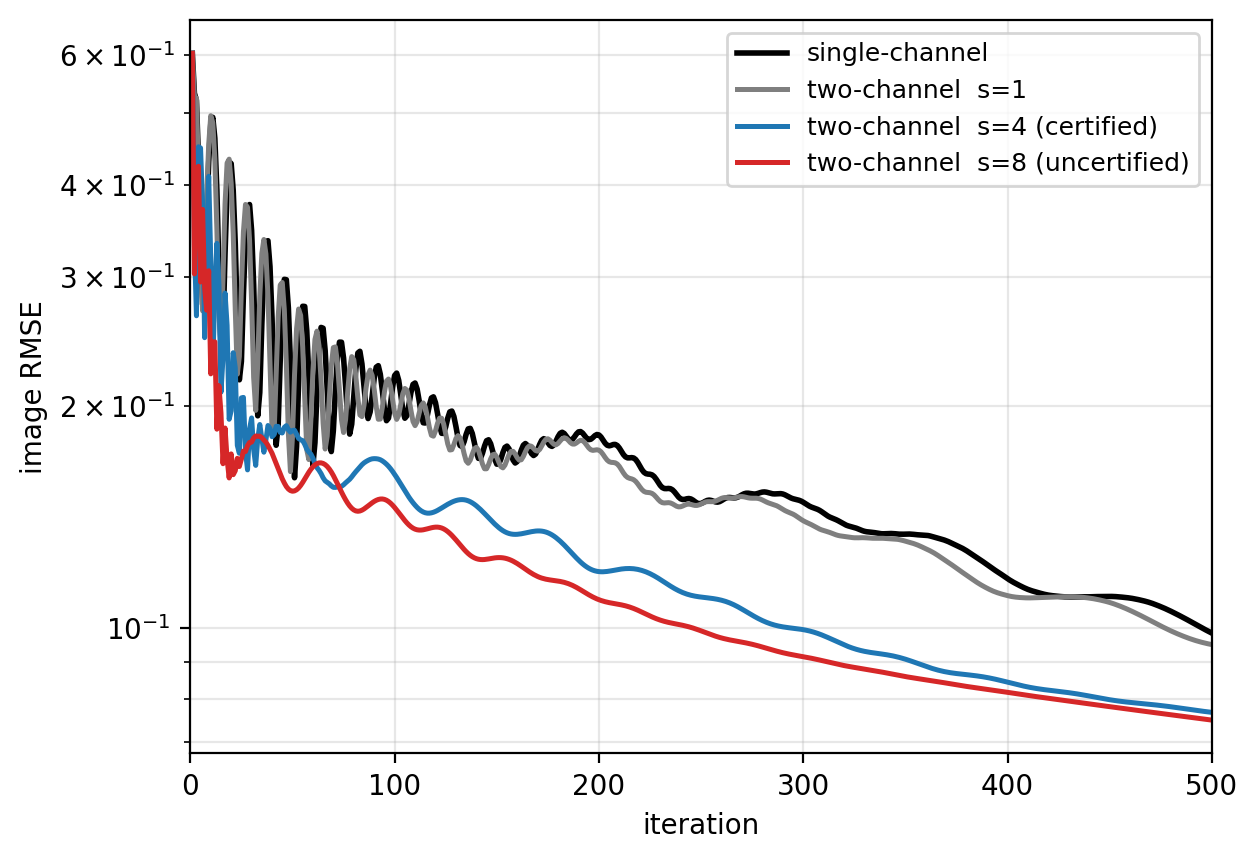
\includegraphics[width=\linewidth]{figs/breast_convergence.png}\\{\small (a) Breast}\end{minipage}\hfill
\begin{minipage}{0.32\linewidth}\centering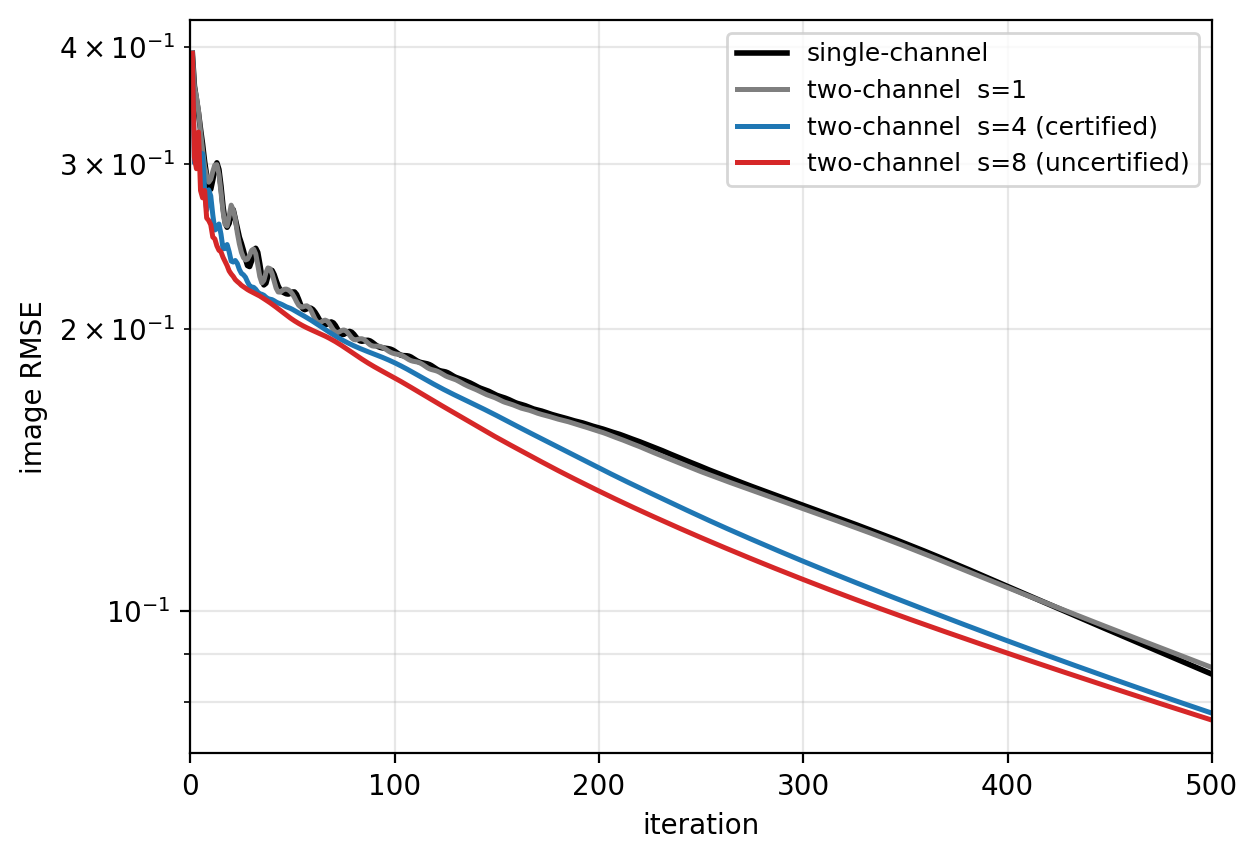
\includegraphics[width=\linewidth]{figs/shepp_logan_convergence.png}\\{\small (b) Shepp--Logan}\end{minipage}\hfill
\begin{minipage}{0.32\linewidth}\centering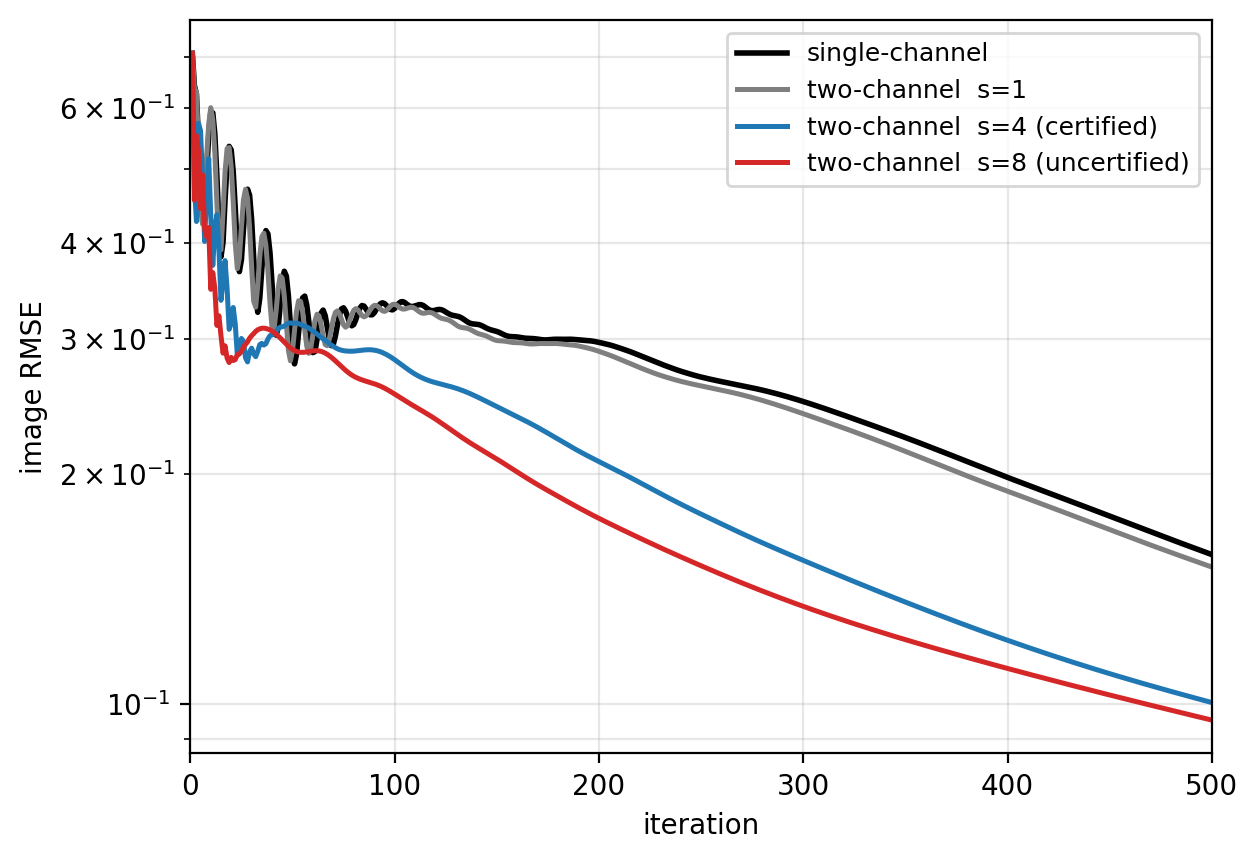
\includegraphics[width=\linewidth]{figs/head_convergence.png}\\{\small (c) Head}\end{minipage}

\medskip
\begin{minipage}{0.32\linewidth}\centering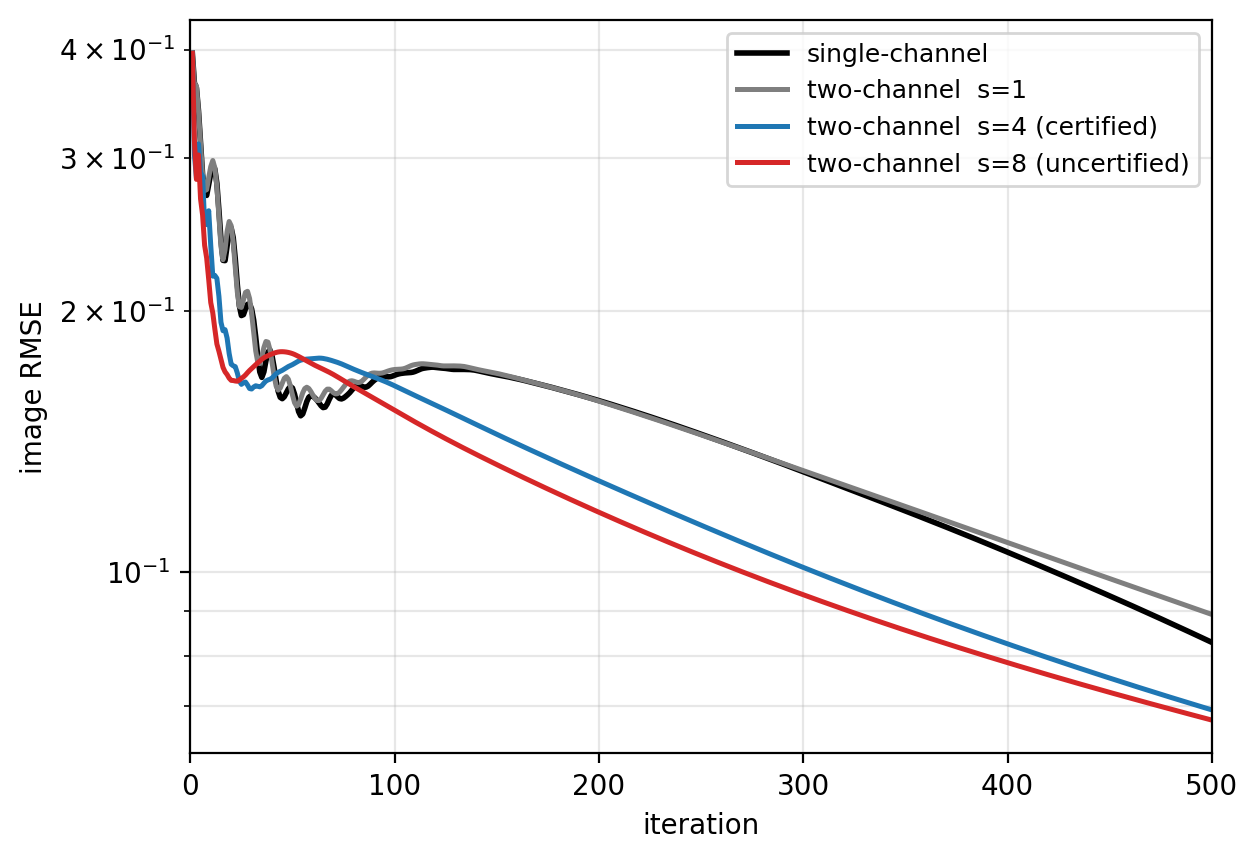
\includegraphics[width=\linewidth]{figs/jaw_convergence.png}\\{\small (d) Jaw}\end{minipage}\hspace{0.03\linewidth}
\begin{minipage}{0.32\linewidth}\centering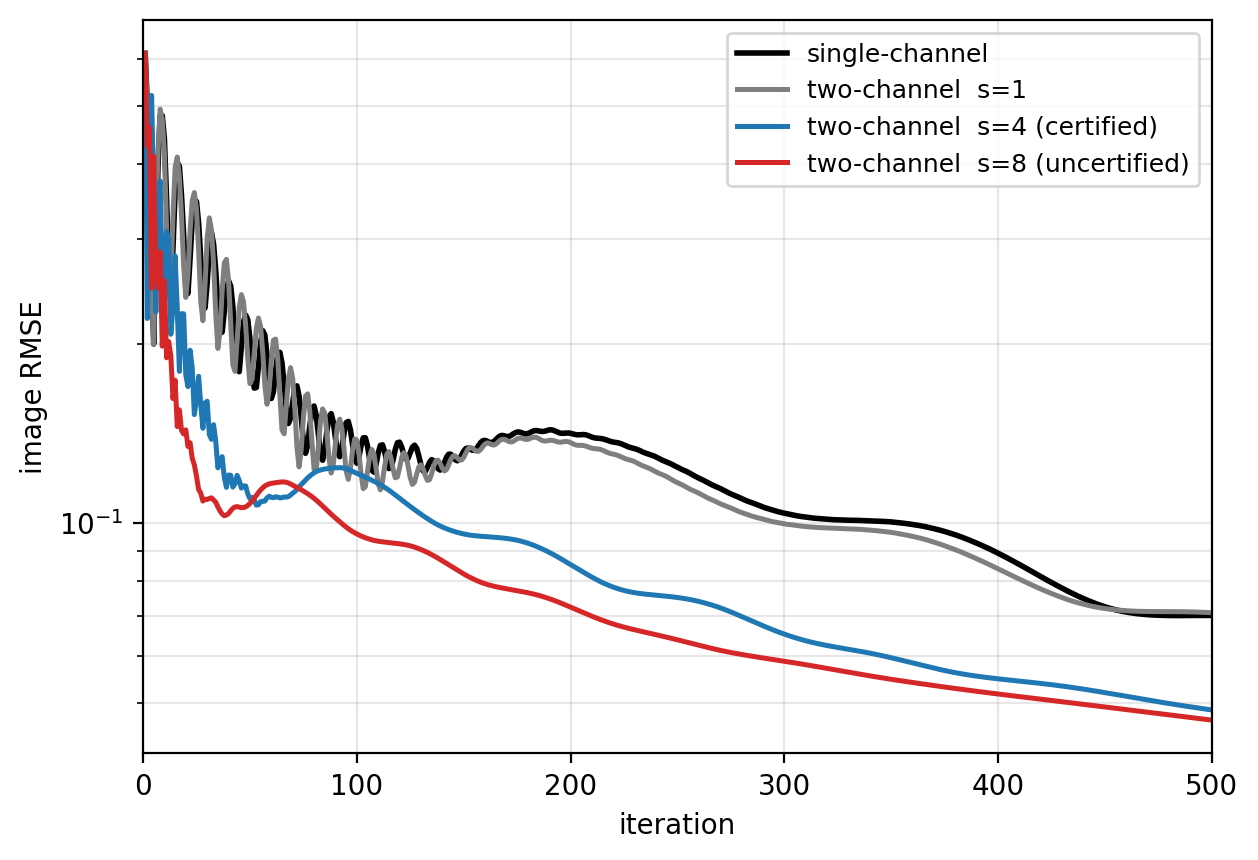
\includegraphics[width=\linewidth]{figs/defrise_convergence.png}\\{\small (e) Defrise}\end{minipage}
\caption{Image RMSE versus iteration for all five phantoms, comparing single-channel reconstruction with the two-channel method at $s\in\{1,4,8\}$.}
\label{fig:conv}
\end{figure}

\begin{figure}[t]
\centering
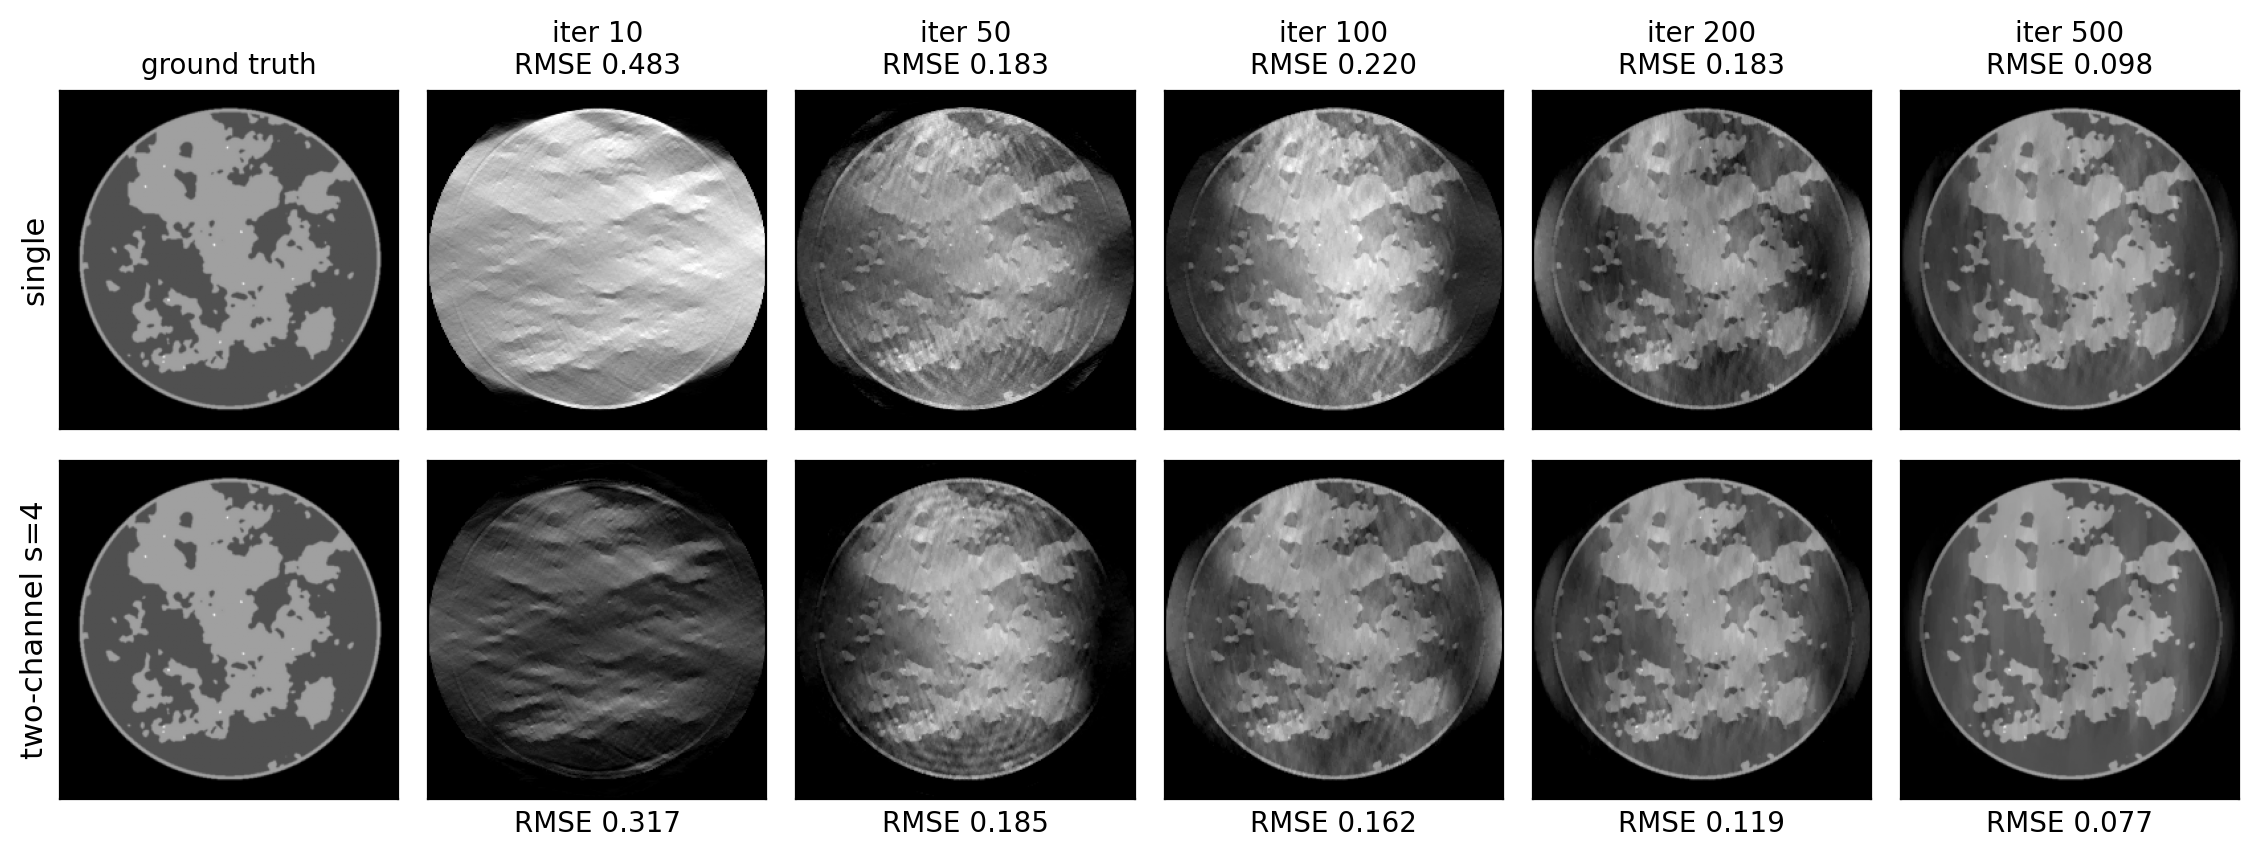
\includegraphics[width=\linewidth]{figs/breast_iter_ladder.png}
\caption{Breast reconstruction at selected iterations: single-channel (top) and two-channel with $s=4$ (bottom). RMSE against the ground truth is annotated for each iterate.}
\label{fig:ladder-breast}
\end{figure}

\begin{figure}[t]
\centering
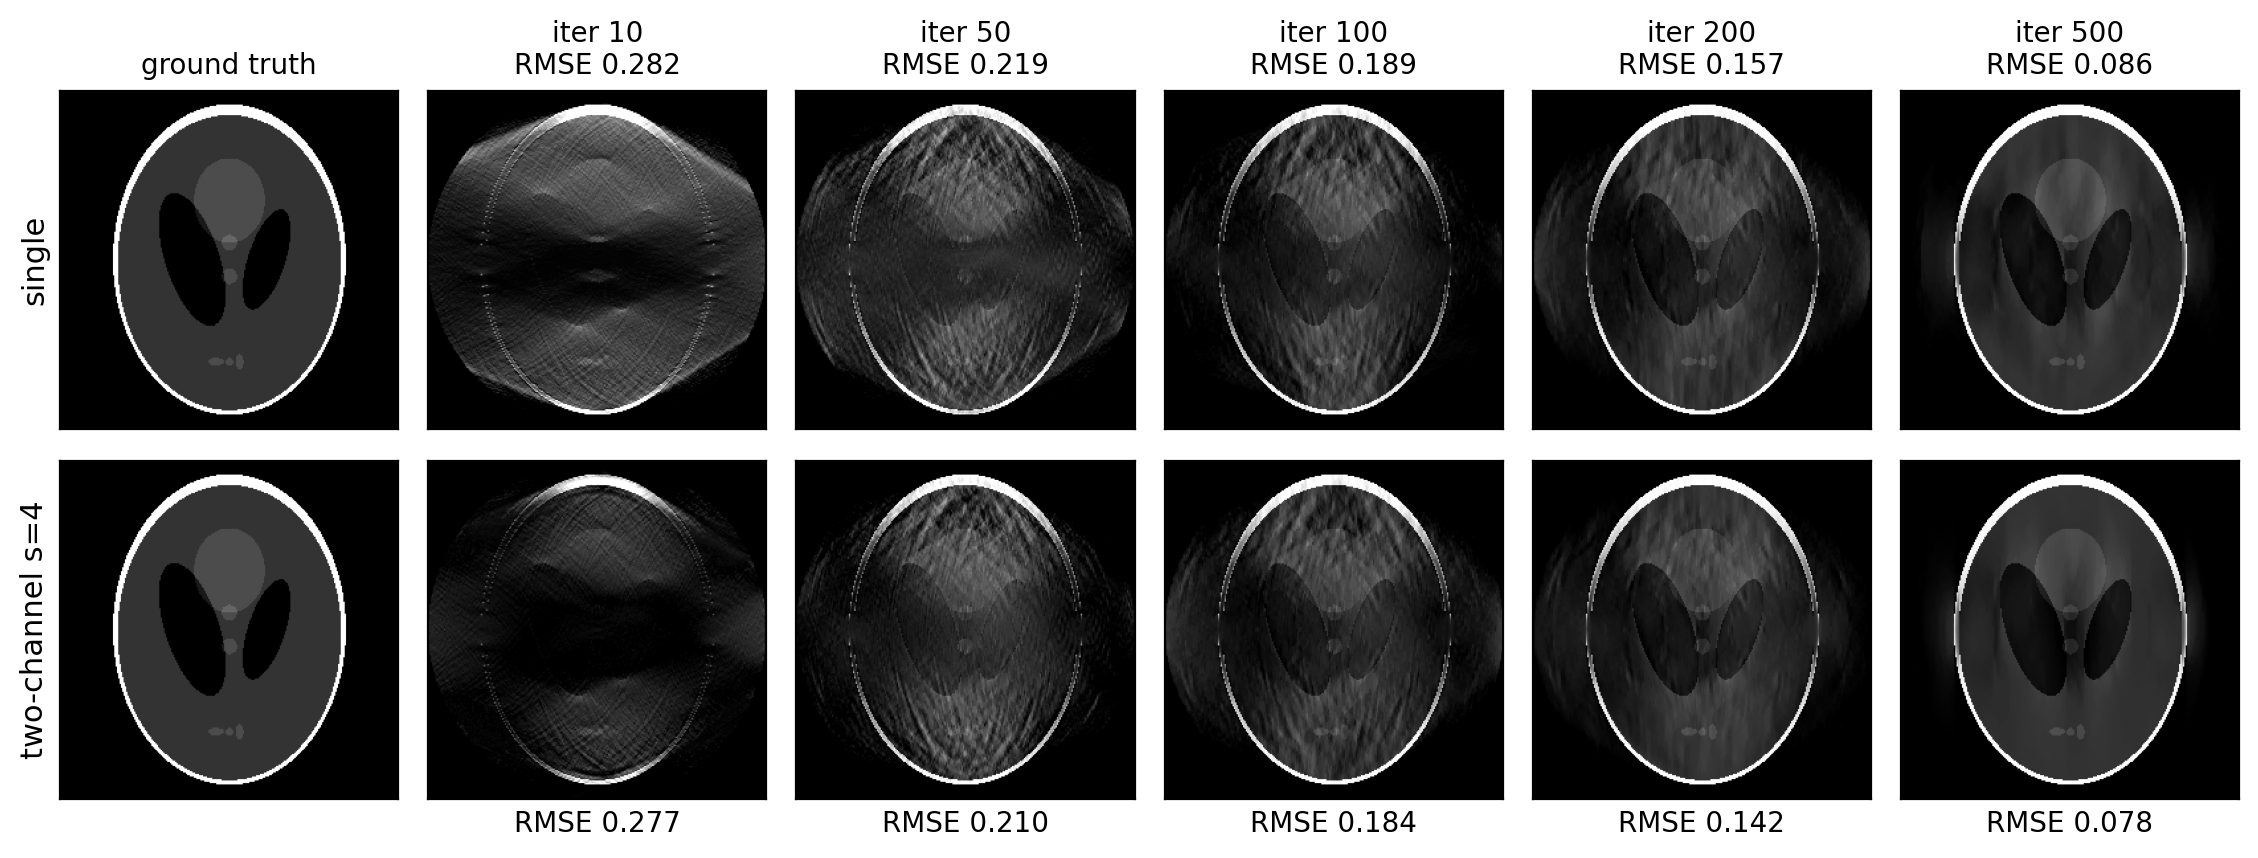
\includegraphics[width=\linewidth]{figs/shepp_logan_iter_ladder.png}
\caption{Shepp--Logan reconstruction at selected iterations: single-channel (top) and two-channel with $s=4$ (bottom), with RMSE annotated.}
\label{fig:ladder-shepp}
\end{figure}

\begin{figure}[t]
\centering
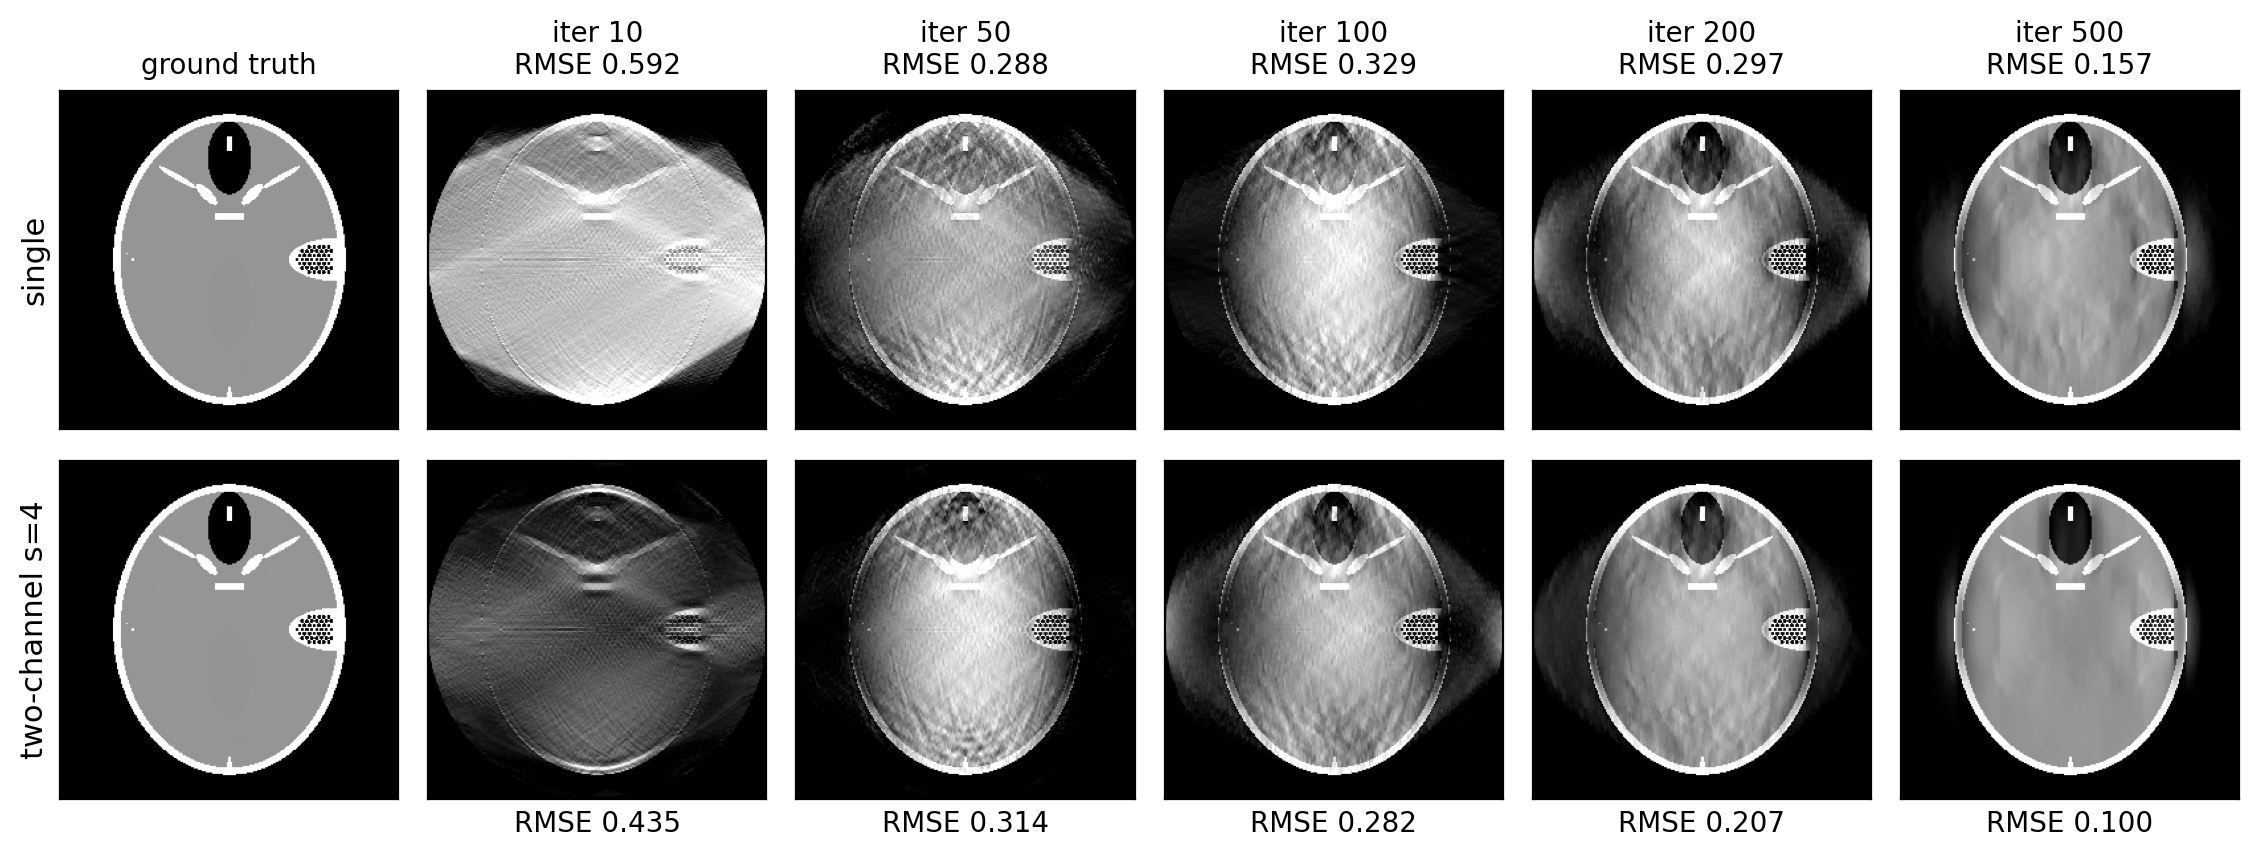
\includegraphics[width=\linewidth]{figs/head_iter_ladder.png}
\caption{Head reconstruction at selected iterations: single-channel (top) and two-channel with $s=4$ (bottom), with RMSE annotated.}
\label{fig:ladder-head}
\end{figure}

\begin{figure}[t]
\centering
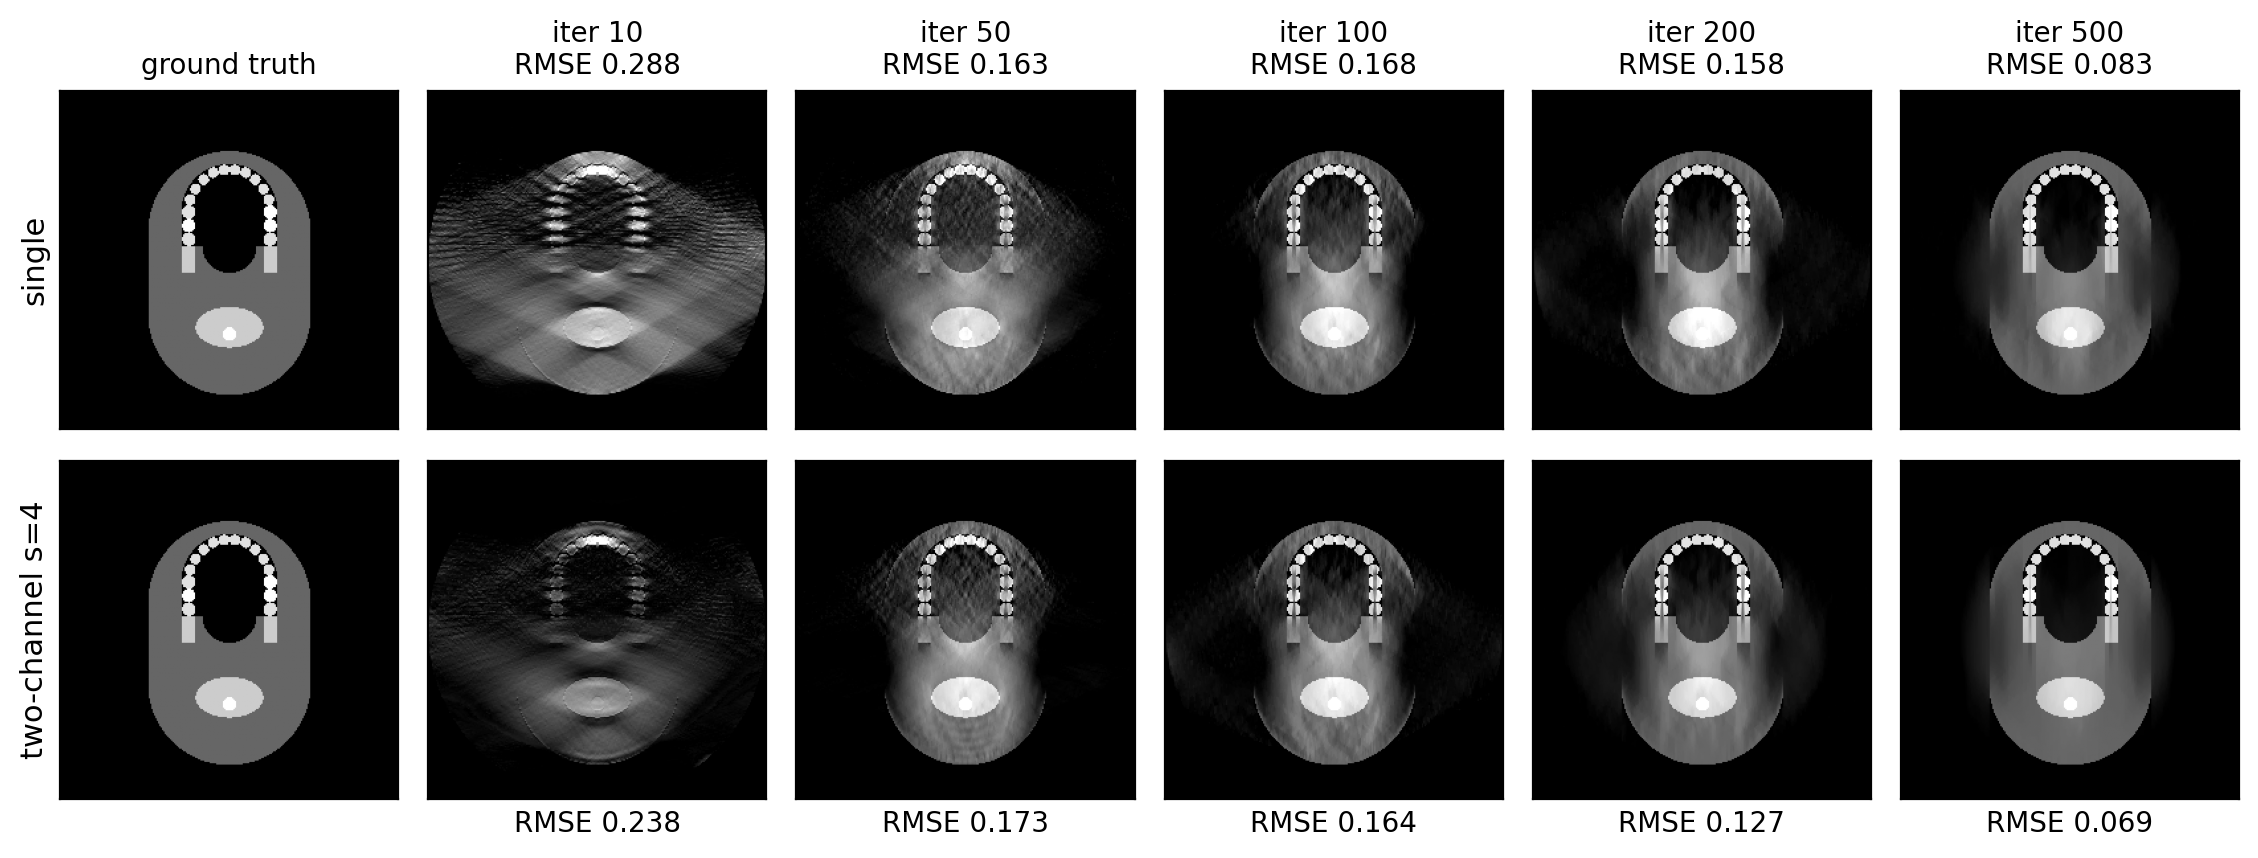
\includegraphics[width=\linewidth]{figs/jaw_iter_ladder.png}
\caption{Jaw reconstruction at selected iterations: single-channel (top) and two-channel with $s=4$ (bottom), with RMSE annotated.}
\label{fig:ladder-jaw}
\end{figure}

\begin{figure}[t]
\centering
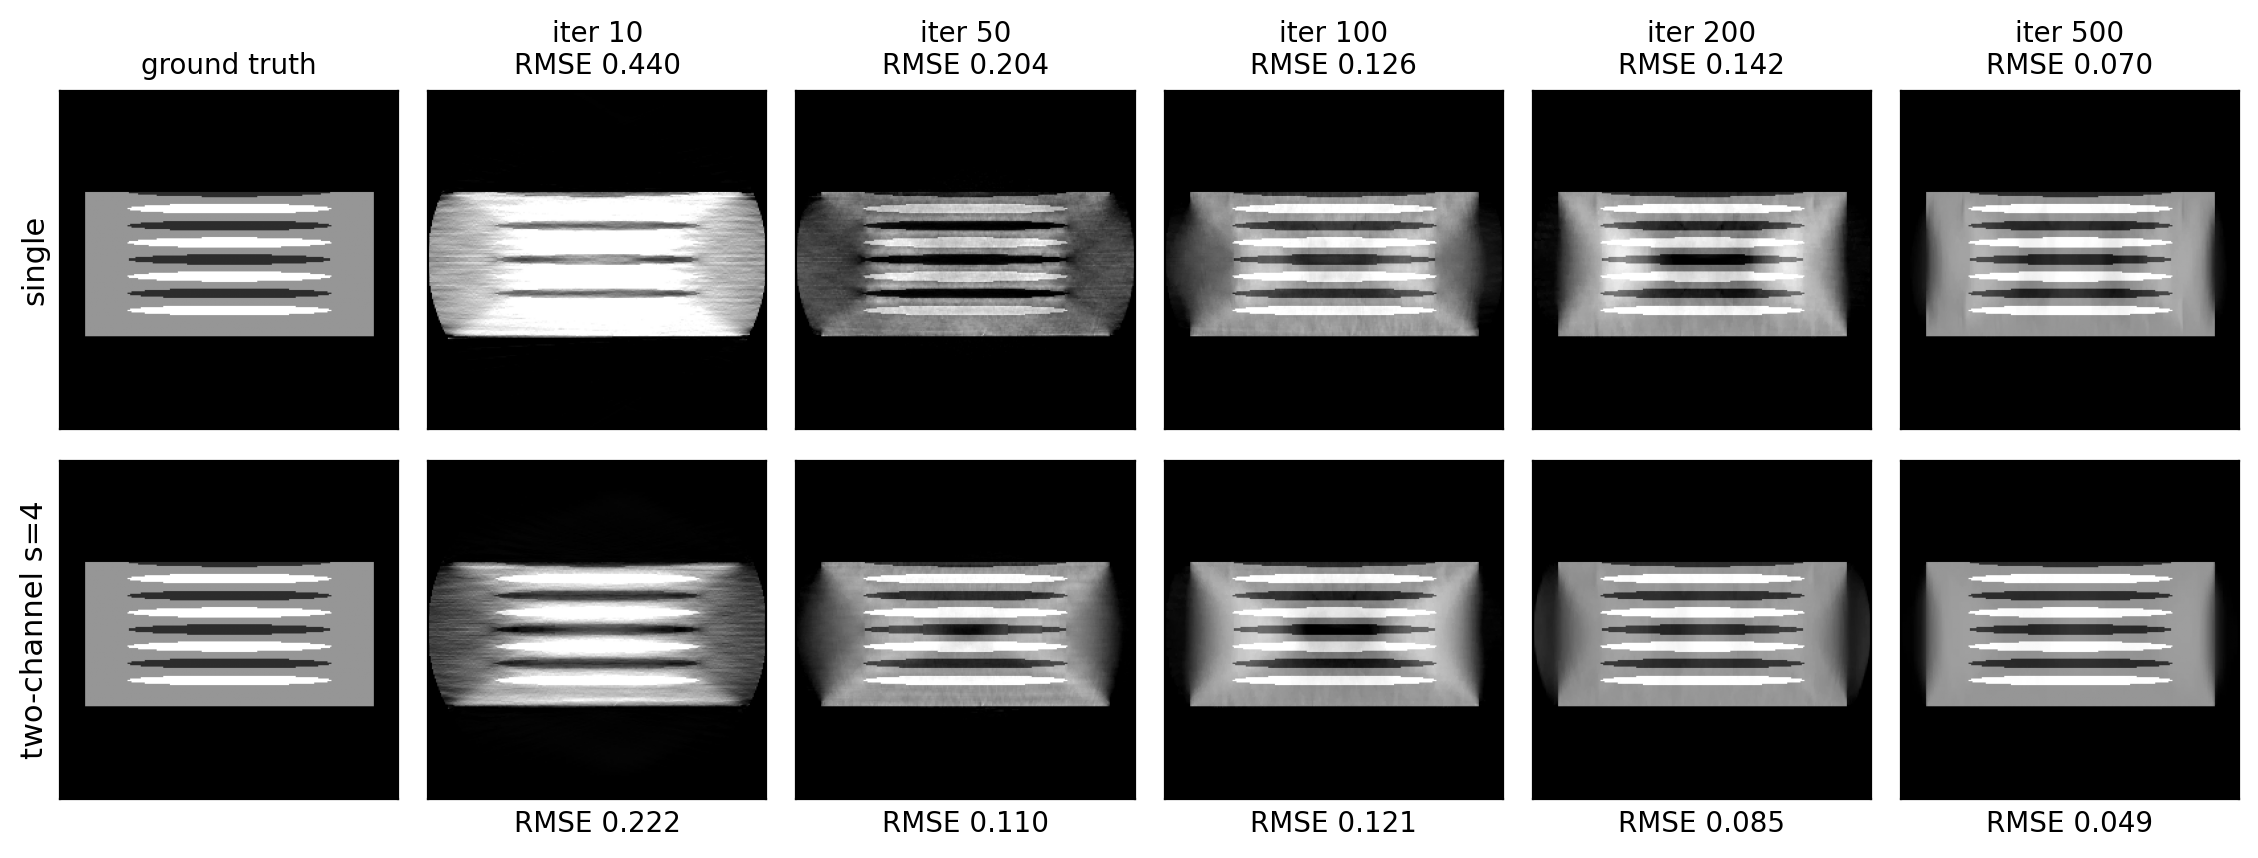
\includegraphics[width=\linewidth]{figs/defrise_iter_ladder.png}
\caption{Defrise reconstruction at selected iterations: single-channel (top) and two-channel with $s=4$ (bottom), with RMSE annotated.}
\label{fig:ladder-defrise}
\end{figure}

\bibliography{references}
\bibliographystyle{abbrvnat}

\end{document}